
\documentclass[10pt]{beamer}

\usetheme{metropolis}

\usepackage{tikz}

\hypersetup{
    colorlinks=true,
    linkcolor=white,
    urlcolor=blue!80
}

\definecolor{uiored}{HTML}{DD0000}
\definecolor{uiolightred}{HTML}{FB6666}
\definecolor{uioredtone}{HTML}{FEE0E0}
\definecolor{uioblue}{HTML}{3E31D6}
\definecolor{uiolightblue}{HTML}{86A4F7}
\definecolor{uioblueone}{HTML}{E6ECFF}
\definecolor{uiogreen}{HTML}{2EC483}
\definecolor{uiolightgreen}{HTML}{6CE1AB}
\definecolor{uiogreentone}{HTML}{CEFFDF}
\definecolor{uioorange}{HTML}{FEA11B}
\definecolor{uiolightorange}{HTML}{FDCB87}
\definecolor{uioorangetone}{HTML}{FFE8D4}
\definecolor{uioyellow}{HTML}{FFFEA7}
\definecolor{uiogray}{HTML}{B2B3B7}

\colorlet{mainbackground}{uiored}

\setbeamercolor{frametitle}{bg=mainbackground, fg=white}
\setbeamercolor{title separator}{fg=mainbackground}
\setbeamercolor{progress bar in section page}{fg=white, bg=uiogray}

\def\logowidth{4cm}

\makeatletter
\setbeamertemplate{section page}
{
  \begingroup

    \vspace{4.3cm}
    {\usebeamercolor[fg]{section title}\usebeamerfont{section title}\insertsectionhead}\\[-1ex]
    {\centering\color{white}\rule{\linewidth}{1pt}\par} % the horizontal line

    \vspace*{3.1cm}
    \begin{center}
        
\includegraphics[width=\logowidth,valign=c]{data/uio_logo_full_white.png} % Adjust width and path to your logo as needed
    \end{center}

  \endgroup
}
\makeatother

\AtBeginSection{
  {
    \setbeamercolor{background canvas}{bg=uiored}
    \setbeamercolor{section title}{fg=white}
    \frame[plain,c,noframenumbering]{\sectionpage}
    \setbeamercolor{background canvas}{bg=black!2}
  }
}

\begin{document}
    \begin{frame}
        \begin{tikzpicture}
            \node[] at (-6, 0) {
                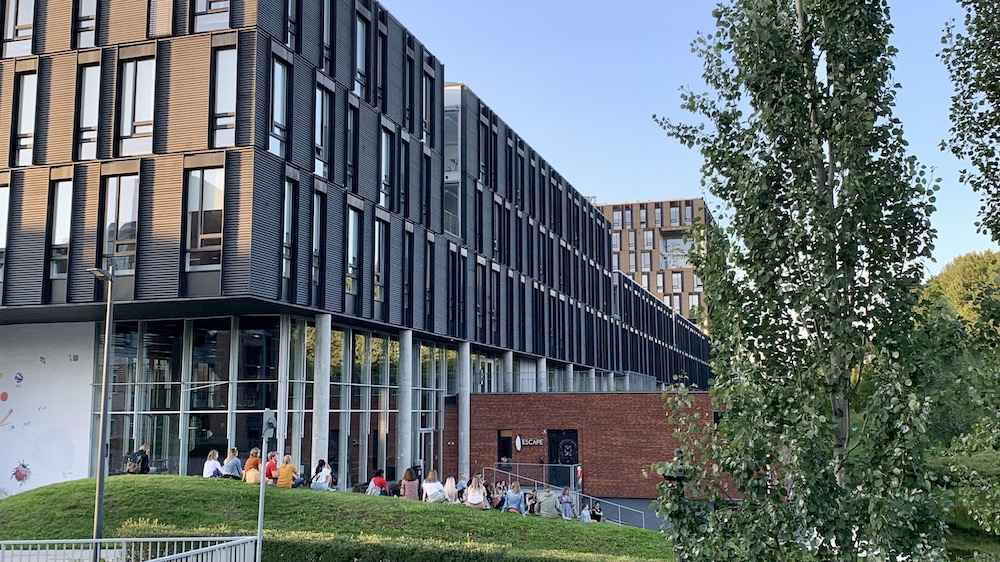
\includegraphics[
                    height=5cm,
                    trim={9cm 0 9cm 0},
                    clip
                ]{data/ifi2.jpg}
            };
            \node[text width=7cm] at (0, 0) {
                \textbf{Utdanning}
                \begin{itemize}
                    \item Mastergrad i Informatikk: Programmering og Nettverk
                    \item Favorittkurs:
                    \begin{itemize}
                        \item Logiske metoder for informatikk
                        \item Logikk og beregninger
                        \item Algoritmer: Design og effektivitet
                        \item Beregnbarhetsteori
                    \end{itemize}
                    \item Jobb som gruppelærer og utvikler
                    \item Var med å starte FIFI
                \end{itemize}
            };
        \end{tikzpicture}
    \end{frame}

    \begin{frame}
        \begin{tikzpicture}
            \node[] at (-6, 0) {
                
\includegraphics[
                    height=5cm,
                    trim={2.32cm 0 2.32cm 0},
                    clip
                ]{data/entrepeneur.png}
            };
            \node[text width=7cm] at (0, 0) {
                \textbf{Start-ups og entrepenørskap}
                \begin{itemize}
                    \item Backend-utvikler i Snapsale
                    \item Lead data scientist og medgründer i Epigram
                    \item Daglig leder og founder i Epigram Medtech
                    \item Styreleder og founder i Biometrical
                    \item Rådgiver og co-founder i SportAI
                    \item CTO og founder i baba.vision
                \end{itemize}
            };
        \end{tikzpicture}
    \end{frame}

    \begin{frame}
        \begin{tikzpicture}
            \node[inner sep=0pt, draw=black] at (-6, 0) {
                
\includegraphics[
                    height=5cm,
                    trim={0.3cm 0 0.3cm 0},
                    clip
                ]{data/paper.png}
            };
            \node[text width=7cm] at (0, 0) {
                \textbf{Forskning}
                \begin{itemize}
                    \item Doktorgrad i kognitiv nevropsykologi
                    \item Post-doc ved Psykologisk institutt/seksjon for presisjonspsykiatri
                    \begin{itemize}
                        \item Analyse av hjernescans med maskinlæring
                        \item Genetikk
                        \item Prediksjon av psykiske lidelser og hjernesykdommer
                    \end{itemize}
                \end{itemize}
            };
        \end{tikzpicture}
    \end{frame}

    \begin{frame}
        \begin{tikzpicture}
            \node[] at (-6, 0) {
                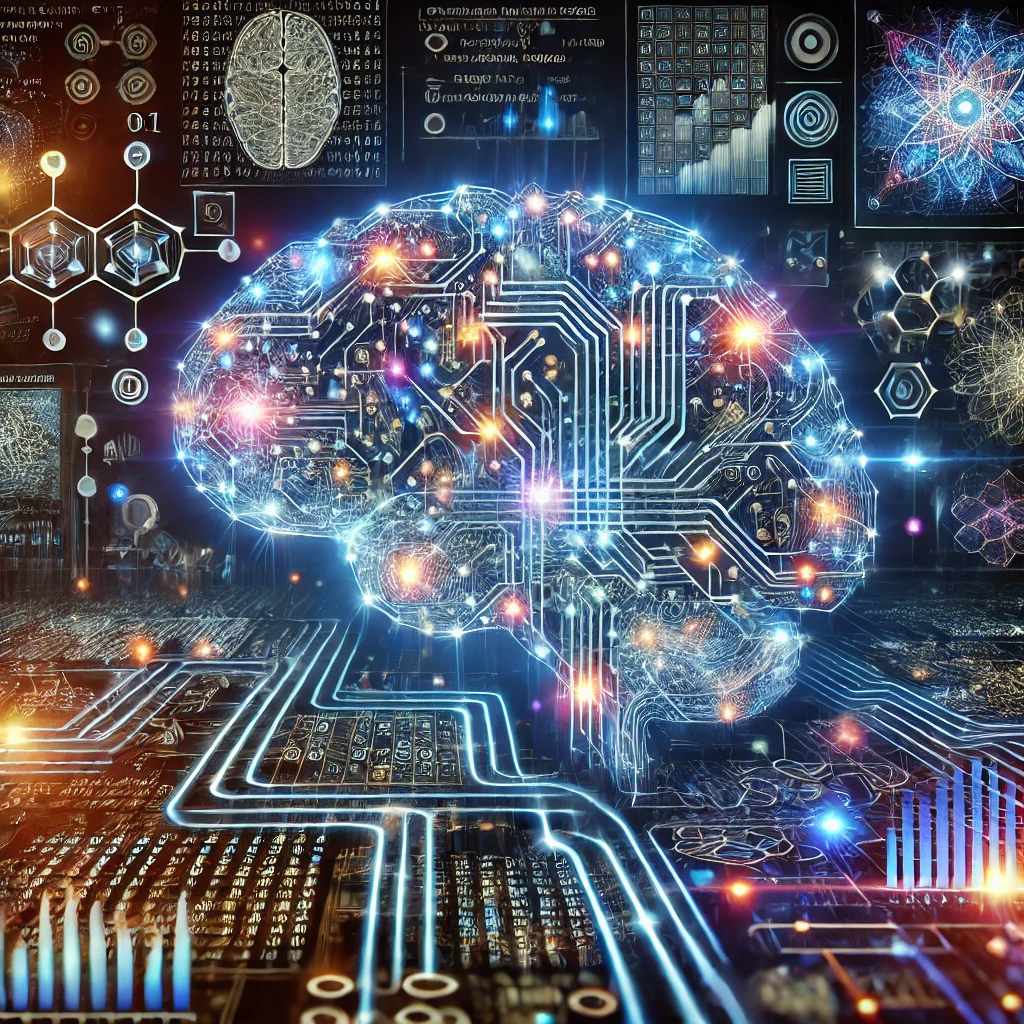
\includegraphics[
                    height=5cm,
                    trim={2.32cm 0 2.32cm 0},
                    clip
                ]{data/ai.png}
            };
            \node[text width=7cm] at (0, 0) {
                \textbf{Faglige interesser}
                \begin{itemize}
                    \item Kunstig intelligens og maskinlæring
                    \item Medisinsk teknologi
                    \item Bevisføring
                    \item Konkurranseprogrammering og -modellering
                \end{itemize}
            };
        \end{tikzpicture}
    \end{frame}
\end{document}
